\section{Renormalization Group, Part IV ($\beta$ Functions)}
\subsection{Review}
Last class got a little bit technical, and this is to a degree unavoidable; the beauty of the renormalization group goes through a path with a lot of technical material (if we want to do anything quantitative with it). Last time, we got up to the point of computing the $\beta$ function for the coupling constants for the effective action. Let us recap this and then go on to discuss how we use these - how we use these is also quite technical, but we will show how to obtain critical exponents from them.

We write the partition function as a certain kind of functional integral:
\begin{equation}
    Z = \int d\phi(x)e^{-S_{\text{eff}}[\phi]}
\end{equation}
which is the same as the old partition function up to a constant; but since we are only interested in calculating correlation functions in the $\phi$s (where the constants will cancel) and the critical behaviour near the phase transition (where since the constant is non-singular in the temperature, it will not contribute), we can neglect the constants in our discussion.

We consider dimensions near 4; $D = 4 - \e$. Our effective action is:
\begin{equation}\label{eq-oldtheory}
    S_{\text{eff}}[\phi] = \int d^{4-\e}x \left(\frac{1}{2}(\nabla \phi(x))^2 + \frac{\tau}{2}\phi^2(x) + \frac{\lambda}{4!}\phi^4\right)
\end{equation}
the argument to get this was follows; we considered an expansion in local operators, and then found that most of these were irrelevant (they could be scaled arbitrarily close to zero). What we have kept are the relevant and marginal operators. Right at $D = 4$, the $\phi^2$ is relevant and $(\nabla \phi)^2$ and $\phi^4$ are marginal. Relevant means they grow under scaling, marginal means they are unchanged under scaling. However note that the fact that the $\phi^2$ gets large here is OK; no matter how much $\tau$ wants to grow, we can tune it to a regime where it does not grow.

We use the word ``operator'' here even though this is all classical statistical mechanics. The sense in which they are is that $\phi$ is really a random variable. And in that sense, you can think of taking correlators of $\phi$ like taking expectation values of operators in quantum mechanics. 

It is also worth pointing out the striking similarity to functional integrals we have seen in quantum field theory. The primary difference; QFT lives in minkowski space where $x_ix^i = -x_0^2 + x_1^2 + x_2^2 + x_3^3$ (with $x_0$ the time coordinate) but here everything is Euclidean.

Another comment; we are analyzing the Ising model, but very little of the Ising model survives here. Although little survives, that which does is quite important. The dimension $D$ remains as a parameter. Another thing is the $\ZZ_2$ symmetry; the theory is unchanged under interchange of $\phi \leftrightarrow -\phi$. Finally, the fact that the interactions are local are encoded in the theory here (although it is hard to see). Note that this technique also predicts the correct universality class for the Ising model.

Last time, we talked about studying this theory, and we have learned that pure perturbation theory (that is - a straightforward saddle point evaluation of the integral) would not work. This is because the terms of order $\lambda$ becomes singular as the temperature is tuned to the critical temperature. The terms of order $\frac{1}{\lambda}$ are mean field. Straightforwards calculation is not in the cards for us. So we take a different route - to somehow figure out how $\lambda$ changes as we do another renormalization group transformation. Now, there is no reason staring at this equation we should expect this to work. If we integrate out the large wavenumber components and do another renormalization group transformation defining an effective action fro the small wavenumbers, $\lambda$ tends to grow (and this can be ascertained via dimensional analysis only). But there are also corrections; the new $\lambda$ is a function of the old one, and it is not linear; these nonlinearities tend to push $\lambda$ to decrease. At some point these two should balance.

\subsection{Another round of RG}
So -  We take our theory and break up $\phi$ into large and small wavenumber components:
\begin{equation}
    \phi = \phi_<(x) + \phi_>(x)
\end{equation}
\begin{equation}
    \int d\phi(x)\ldots = \int d\phi_<(x)d\phi_>(x)\ldots
\end{equation}
This sort of calculation - the bad parts of PT does not hold as the integration over the large wavenumbers does not produce a singularity. This becomes an exercise in doing a Gaussian integral, out of which we get another effective action:
\begin{equation}
    S_{\text{eff}}[\phi_< + \phi_>] = S_{\text{eff}}[\phi_<] + \int d^{4-\e}x\left(\frac{1}{2}(\nabla \phi_>)^2 + \frac{\tau}{2}\phi_>^2 + \frac{\lambda}{2}\phi_<^2\phi_>^2\right) + \ldots
\end{equation}
We're now doing an expansion in $\lambda$; so truncating is a consistent to do. Now, doing an integral in $\phi_>$ is just the familiar Gaussian integral - we then obtain:
\begin{equation}
    \int d^{4-\e}x \left(\frac{1}{2}(\nabla \phi_<)^2 + \frac{\tau}{2}\phi_<^2 + \frac{\lambda}{4!}\phi_<^4\right) + \frac{1}{2}\Tr\ln(-\nabla^2 + \tau + \frac{\lambda}{2}\phi_<^2) + \ldots
\end{equation}
this is not yet quite $S_{\text{eff}}$ as we are yet to do the rescaling. So now, there are a few things left to do. First, we have to evaluate the above; this seems impossible but maybe there is something we can do. Then there is the scaling transformation. For the old theory, in Eq. \eqref{eq-oldtheory}, our cutoff was $\abs{p} = 1$:
\begin{equation}
    \phi(x) = \int_{\abs{p} < 1} \frac{d^{4-\e}p}{(2\pi)^{4-\e}}e^{ip \cdot x}\phi(p)
\end{equation}
So in the $\phi_>$ integral , we took $\Lambda \leq \abs{p} < 1$, and in the $\phi_>$ integral we took $0 \leq \abs{p} \leq \Lambda$. So $\phi_<$ has ``cutoff'' $\Lambda$. We now rescale things so the cutoff is set back to $1$. We then get a new $\lambda$ and new $\tau$, and we do this to learn what the new $\lambda/\tau$ look like as a function of the old.

\subsection{Computing Corrections}
Now, $-\nabla^2 + \tau + \frac{\lambda}{2}\phi_<^2$ is a differential operator, which we can view as a matrix on function space:
\begin{equation}
    (-\nabla^2 + \tau + \frac{\lambda}{2}\phi_<^2)\delta(x-y)
\end{equation}
to calculate the trace log, the only way forwards is to find the eigenvalues of the matrix. Then, the log of the matrix is just the matrix with the log eigenvalues. But this is of course impossible as the matrix contains an arbitrary function $\phi_<$. So, what to do? What I am really interested in is how the matrix depends on $\phi_<$. So, I could for example do perturbation theory in $\phi_<$. So, let's have a look at that.

To zeroth order, we have:
\begin{equation}
    \Tr(\ln(-\nabla^2 + \tau + \frac{\lambda}{2}\phi_<^2)) = \Tr(\ln(-\nabla^2 + \tau))
\end{equation}
by setting $\phi_< = 0$. But this just gives a $\phi_<$ independent constant in our action, so we can neglect it (and don't have to worry about evaluating). To the next order, we have:
\begin{equation}
    \Tr(\ln(-\nabla^2 + \tau + \frac{\lambda}{2}\phi_<^2)) = \Tr(\ln(-\nabla^2 + \tau)) + \Tr(\ln(1 + \frac{1}{-\nabla^2 + \tau}\frac{\lambda \phi_<^2}{2}))
\end{equation}
which we can then do a power series expansion in the logarithm:
\begin{equation}
    \Tr(\ln(-\nabla^2 + \tau + \frac{\lambda}{2}\phi_<^2)) = \Tr(\ln(-\nabla^2 + \tau)) + \Tr\frac{1}{-\nabla^w + \tau}\frac{\lambda \phi_<^2}{2} - \frac{1}{2}\Tr(\frac{1}{-\nabla^2 + \tau}\frac{\lambda \phi_<^2}{2}\frac{1}{-\nabla^2 + \tau}\frac{\lambda\phi_<^2}{2}) + \ldots
\end{equation}
where note by the cyclicity of the trace the order of the operators appearing in the last term does not matter (even if they do not commute).
We can neglect about the higher order terms as they will scale to zero. Dropping the first term:
\begin{equation}
    \Tr(\ln(-\nabla^2 + \tau + \frac{\lambda}{2}\phi_<^2)) = \Tr\frac{1}{-\nabla^w + \tau}\frac{\lambda \phi_<^2}{2} - \frac{1}{2}\Tr(\frac{1}{-\nabla^2 + \tau}\frac{\lambda \phi_<^2}{2}\frac{1}{-\nabla^2 + \tau}\frac{\lambda\phi_<^2}{2})
\end{equation}
Now, let's analyze what we have:
\begin{equation}
    \Tr\frac{1}{-\nabla^2 + \tau}\frac{\lambda \phi_<^2}{2}
\end{equation}
the first term is:
\begin{equation}
    \int d^{4-\e}y \left(\frac{1}{-\nabla^2 + \tau}\right)\delta(x - y) = \int d^{4-\e}y \frac{d^{4-\e}p}{(2\pi)^{4-\e}}\frac{e^{ip(x-y)}}{p^2 + \tau}
\end{equation}
and the second term is:
\begin{equation}
    \lim_{z \to x}\int d^{4-\e}y\frac{\lambda}{2}\phi_<^2(y) \delta(y - z)
\end{equation}
So:
\begin{equation}
    \int d^{4-\e}x \int d^{4-\e}y \int \frac{d^{4-\e}p}{(2\pi)^{4-\e}}\frac{e^{ip(x-y)}}{p^2 + \tau}
\end{equation}
so at the end of the day we have:
\begin{equation}
    \left(\int \frac{d^{4-\e}p}{(2\pi)^{4-\e}}\frac{1}{p^2 + \tau}\right)\int d^{4-\e}\frac{\lambda}{2}\phi_<^2(y)
\end{equation}
so here, we have found exactly the coefficient for the correction to  $\phi_<^2$. We can proceed and do the same for the $\phi_<^4$ term. And we can then go ahead and obtain a new theory, i.e. a new effective action. Our scaling is:
\begin{equation}
    \phi(x) \to \Lambda^{\frac{2 - \e}{2}}\phi(\Lambda x)
\end{equation}
which sets $\Lambda \to 1$, and we get a new effective action:
\begin{equation}
    S_{\text{eff}}[\phi] = \int\left(\frac{1}{2}(\nabla \phi)^2 + \frac{\tilde{\tau}}{2}\phi^2 + \frac{\tilde{\lambda}}{4!}\phi^4\right)
\end{equation}
where we drop the $<$ on the $\phi$s. The new $\tilde{\tau}/\tilde{\lambda}$s are:
\begin{equation}
    \tilde{\tau} = \frac{\tau}{\Lambda^2} + \frac{\lambda}{32\pi^2}\left[\left(\frac{1}{\Lambda^2} - 1\right) - \frac{\tau}{\Lambda^2}\ln\frac{1 + \tau}{\Lambda^2 + \tau}\right]
\end{equation}
so we get something whose size is controlled by $\lambda$ and depends on $\Lambda, \tau$. In a way, this is a correction to $T_c$. We can also do the integrals for the fourth order terms:
\begin{equation}
    \tilde{\lambda} = \lambda - \e\lambda \ln\Lambda - \frac{3}{32\pi^2}\lambda^2\left[\ln\frac{1+\tau}{\Lambda^2 + \tau} - \tau\left(\frac{1}{\Lambda^2 + \tau} - \frac{1}{1 + \tau}\right)\right]
\end{equation}
which is the endpoint of some awful integrals. 

\subsection{Evolution of the Theory}
So, we can now see how our theory evolves:
\begin{equation}
    \left.\Lambda\dpd{}{\Lambda} \tilde{\lambda}(\Lambda)\right|_{\Lambda =1} = -\e\lambda + \frac{3}{32\pi^2}\lambda^2
\end{equation}
\begin{equation}
    \left.\Lambda\dpd{}{\Lambda} \tilde{\tau}(\Lambda)\right|_{\Lambda =1} = -2\tau - \frac{\lambda}{16\pi^2}
\end{equation}
Here we see the balance of $\lambda$ being pushed to increase/decease. If we think of this as a flow (and there is a good reason to think of this in that way) then the LHS is the rate of the flow, and the sign of the RHS gives the direction. If I plot the RHS, which we call $\beta(\lambda)$, we get:
\begin{figure}[htbp]
    \centering
    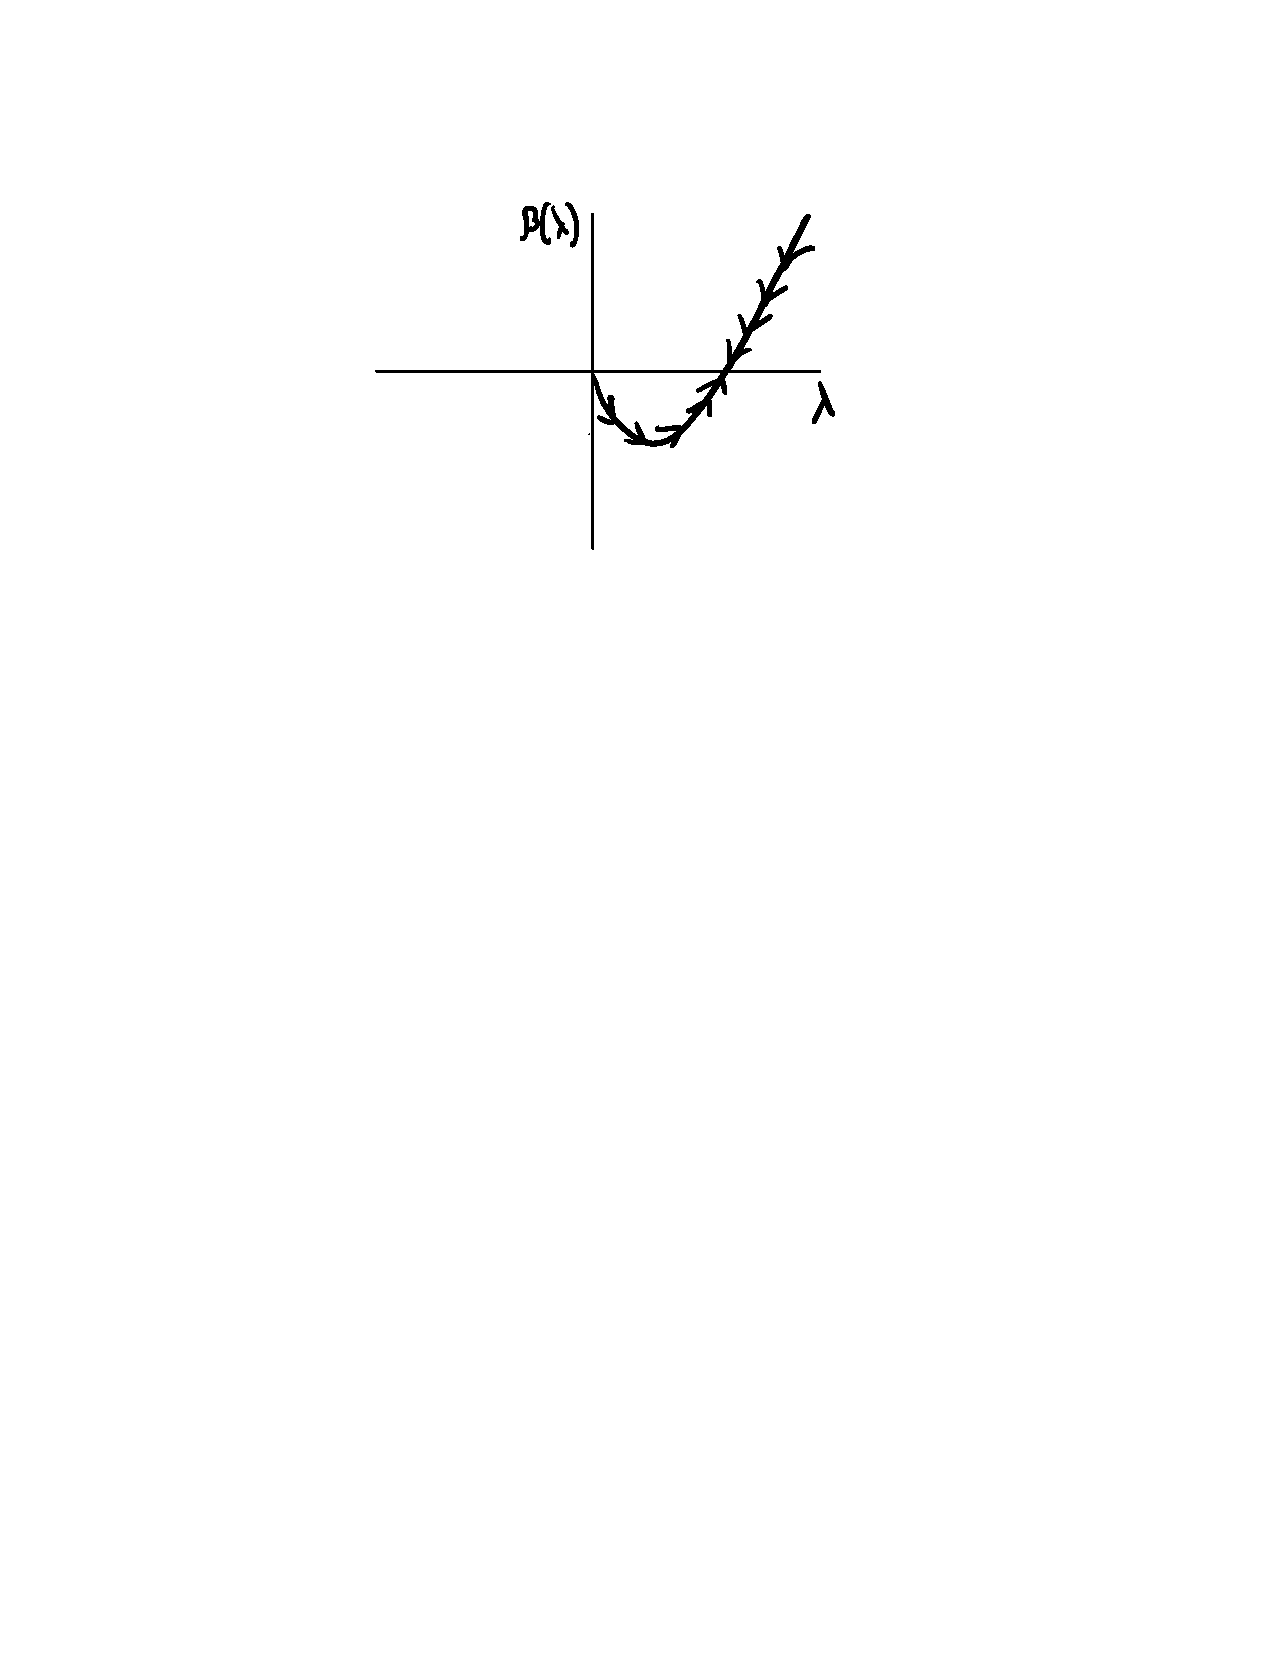
\includegraphics[scale=0.7]{Images/fig-betaplot2.pdf}
    \caption{Graph of $\beta$ function.}
    \label{fig-betaplot2}
\end{figure}
so wherever I start with $\lambda$, the RG pushes it towards the Wilson-Fisher fixed point. This is an attractor, which should determine in some sense the physics of this model. Also notice that $\lambda \neq 0$ here, so the model is intrinsically interacting. Note the reason why this program succeeds is that the Wilson-Fisher fixed point is isolated, which we will see the reason for in a future lecture.

Note that until the conformal bootstrap was invented, fancy asymptotic techniques of setting $\e = 1$ was considered the systematic solution to second order phase transitions. 

This has been technical - going through it maybe we are a bit dissapointed. Something so powerful shouldn't be so technical. This might mean that there are still ideas to be had, to understand the parts of this that are mathematical and not very physical. 

Next time, we go through how to use this to calculate critical exponents. Note that perturbation theory will not work for this. Perturbation theory will be ruined by the scaling as we come up to the phase transition point (as we expand around MFT which is less singular than the perturbations). What we will need is to look at the renormalization group.